%
% File acl2014.tex
%
% Contact: koller@ling.uni-potsdam.de, yusuke@nii.ac.jp
%%
%% Based on the style files for ACL-2013, which were, in turn,
%% Based on the style files for ACL-2012, which were, in turn,
%% based on the style files for ACL-2011, which were, in turn, 
%% based on the style files for ACL-2010, which were, in turn, 
%% based on the style files for ACL-IJCNLP-2009, which were, in turn,
%% based on the style files for EACL-2009 and IJCNLP-2008...

%% Based on the style files for EACL 2006 by 
%%e.agirre@ehu.es or Sergi.Balari@uab.es
%% and that of ACL 08 by Joakim Nivre and Noah Smith

\documentclass[11pt]{article}
\usepackage{acl2014}
\usepackage{times}
\usepackage{url}
\usepackage{latexsym}


%%%%%% ADDED TO GET CORRECT PDF SIZE
\pdfpagewidth=\paperwidth
\pdfpageheight=\paperheight


%%%%%% EXTRA PACKAGES
\usepackage{graphicx}
\usepackage{listings}
\usepackage{tabularx}
\usepackage{ctable}
\usepackage{booktabs}


%\setlength\titlebox{5cm}

% You can expand the titlebox if you need extra space
% to show all the authors. Please do not make the titlebox
% smaller than 5cm (the original size); we will check this
% in the camera-ready version and ask you to change it back.


\title{\textit{lex4all}: A language-independent tool for building and evaluating pronunciation lexicons for small-vocabulary speech recognition}

%\author{Anjana Vakil \\
%  Affiliation / Address line 1 \\
%  Affiliation / Address line 2 \\
%  Affiliation / Address line 3 \\
%  {\tt email@domain} \\\And
%  Max Paulus \\
%  Affiliation / Address line 1 \\
%  Affiliation / Address line 2 \\
%  Affiliation / Address line 3 \\
%  {\tt email@domain} \\}

\date{}

\begin{document}
\maketitle

\begin{abstract}
This paper describes \textit{lex4all}, an open-source PC application for the generation and evaluation of pronunciation lexicons in any language. With just a few minutes of recorded audio and no expert knowledge of linguistics or speech technology, individuals or organizations seeking to create speech-driven applications in low-resource languages can use this tool to build pronunciation lexicons enabling small-vocabulary speech recognition in the target language using a high-quality commercial recognition engine designed for a high-resource source language (e.g. English). This is possible thanks to an existing algorithm for cross-language phoneme-mapping; we give an overview of this method and describe its implementation in \textit{lex4all}. Beyond the core functionality of building new lexicons, the tool also offers a built-in audio recorder that facilitates data collection, and an evaluation module that simplifies and expedites research on small-vocabulary speech recognition using cross-language mapping. 
%Finally, we report on an investigation into the impact of varying the high-resource source language used; our results seem to indicate that phonetic similarity between target and source language does not significantly affect recognition accuracy, underscoring the system's language-independence.
\end{abstract}


%Demo submissions should also clearly indicate if any computer equipment is expected to be provided by the local organizer. If so, please specify desired hardware platform, hard disk and memory capacity, operating system and other software needed in order to run the demo. 
%
%Implementation of ACL multiple submission policy: Papers being submitted both to ACL and another conference or workshop must
%\begin{itemize}
%\item Note on the title page the other conference or workshop to which they are being submitted. (This includes submissions that are extensions of papers currently being submitted to a workshop.)
%\item State on the title page that if the paper is accepted for ACL, then the paper will be withdrawn from other conferences and workshops.
%\end{itemize}
%Papers that overlap other papers that have appeared at a conference with published proceedings must contain significant new results. Authors must include on the title page a list of any previous papers that the current paper overlaps or extends, and must identify the significant new results contained in the new submission. The program co-chairs have the final decision about what constitutes significant new results.

\section{Introduction\footnote{Parts of this paper (Sections \ref{sec:intro} and \ref{sec:background}) overlap with a paper submitted to the 4th Workshop on Spoken Language Technologies for Under-resourced languages (SLTU '14, \url{http://www.mica.edu.vn/sltu2014}). That paper, which is currently under review, concerns related research not reported here, and makes no mention of the lex4all application.}}
\label{sec:intro}

In recent years it has been demonstrated that speech recognition interfaces can be extremely beneficial for applications in the developing world, particularly in communities where literacy rates are low or where PCs and internet connections are not always available \cite{case4st4d,bali13,Sherwani09}. 
Typically, the languages spoken in such communities are under-resourced, such that the large audio corpora typically needed to train or adapt recognition engines are unavailable.
%, and collecting such vast amounts of data is generally infeasible for individuals or small organizations interested in developing speech-driven applications for their communities. 
However, in the absence of a recognition engine trained for the target low-resource language (LRL), an existing recognizer for a completely unrelated high-resource language (HRL), such as English, can be used to perform small-vocabulary recognition tasks in the LRL. 
%(By ``small-vocabulary tasks'' we mean those requiring discrimination between a few dozen terms.) 
%of the type required in grammar-controlled applications (e.g. for accessing information or conducting basic transactions), which may require the system to distinguish a few dozen terms in the URL. 
All that is needed is a pronunciation lexicon mapping each term in the target vocabulary to one or more sequences of phonemes in the HRL, i.e. phonemes which the recognizer can model. 

This is the motivation behind \textit{lex4all},\footnote{[Link removed to preserve submission anonymity]} an open-source desktop application for Windows that allows users to automatically create a mapped pronunciation lexicon for words in any language, using a small number of audio recordings and a pre-existing recognition engine in a HRL such as English. The resulting lexicon can then be used with the HRL recognizer to add small-vocabulary speech recognition functionality to applications in the LRL, without the need for the large amounts of data and expertise in speech technologies required to train a new recognizer. This paper describes the \textit{lex4all} application and its utility as a tool for rapid, simple creation and evaluation of mapped pronunciation lexicons for small-vocabulary speech recognition in any language.

\section{Background and related work}
\label{sec:background}
Many commercial speech recognition systems offer high-level Application Programming Interfaces (APIs) that make adding voice recognition capabilities to an application as simple as specifying (in text) the words/phrases that should be recognized; this requires very little general technical expertise, and virtually no knowledge of the inner workings of the recognition engine. If the target language is supported by the system -- the Microsoft Speech Platform, for example, currently supports recognition and synthesis for 26 languages/dialects \cite{mspsdk} -- this makes it very easy for small-scale software developers (i.e. individuals or small organizations without much funding) to create new speech-driven applications. 

While many such individuals or organizations in the developing world may be interested in using such platforms to create speech-driven applications for use in their communities, the low-resource languages typically spoken in these areas are obviously not supported by such commercial systems. 
And though many effective techniques for training or adapting recognizers for new languages exist (e.g. CMUSphinx\footnote{\url{http://www.cmusphinx.org}} or the Rapid Language Adaptation Toolkit\footnote{\url{http://i19pc5.ira.uka.de/rlat-dev}}), these typically require hours of training audio to produce effective models, and even the highest-level tools for building new models still require a nontrivial amount of expertise with speech technologies; such data and expertise may not be available to the small-scale developers in question.

However, many useful development-oriented applications (e.g. for accessing information or conducting basic transactions) require only small-vocabulary recognition tasks, by which we mean those requiring discrimination between a few dozen terms.
For such tasks, an unmodified HRL recognizer can be used as-is to perform recognition of the LRL terms; 
%as Figure~\ref{fig:background} illustrates, 
we simply provide the recognizer with an application-specific grammar describing the allowable combinations and sequences of words/phrases to be recognized, and a pronunciation lexicon which maps each of the target words/phrases to a sequence of phonemes in the source language for which the recognizer has been trained. 

%\begin{figure}[tb]
%\begin{center}
%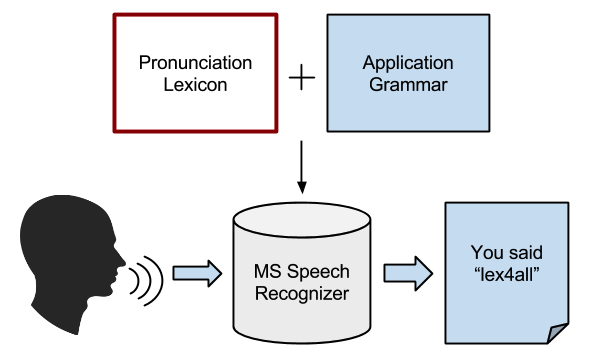
\includegraphics[width=\columnwidth]{../img/background-diagram-cropped.png}
%\caption{Given a pronunciation lexicon and application-specific grammar, an existing recognizer for a HRL can be used to recognize speech in a LRL.\label{fig:background}}
%\end{center}
%\end{figure}



This is the thinking behind Speech-based Automated Learning of Accent and Articulation Mapping, or ``Salaam'' \cite{Sherwani09,Qiao10,Chan12}. This method of cross-language phoneme-mapping enables the automatic discovery of source-language pronunciation sequences for words or phrases in the (unrelated) target language, and 
%thus constitutes the foundation on which the lex4all tool is built.
is the technique at the core of the lex4all lexicon-building tool.

The basic idea of phoneme-mapping is to discover the best pronunciation sequence for a given word in the target language by using the source language recognizer to perform phone decoding on one or more audio samples of the target word. However, the APIs for commercial recognizers such as Microsoft's are designed for word-decoding, and do not usually enable the use of the phone-decoding mode. The insight of the Salaam approach is to use a specially designed grammar 
to mimic phone decoding 
and guide pronunciation discovery 
%THIS CITATION IS HARD-CODED BECAUSE OF MULTIPLE SECTION NUMBERS
(Qiao~et~al., 2010, \S4.1; Chan~and~Rosenfeld, 2012, \S3.2).
%Specifically, Qiao et al. \cite[\S4.1]{Qiao10} create a recognition grammar representing a phoneme ``super-wildcard'' that guides pronunciation discovery. 
This so-called ``super-wildcard'' grammar allows the recognizer to treat an audio sample of the target word as a ``phrase'' made up of 0-10 ``words'',
where each ``word'' can be matched to any possible sequence of 1, 2, or 3 source language phonemes \cite[\S4.1]{Qiao10}. 

Given this super-wildcard grammar and one or more audio recordings of the target word, \newcite[\S4.1]{Qiao10} use an iterative training algorithm to discover the best pronunciation(s) for that word, one phoneme at a time. 
In the first pass, the recognizer finds the best match(es) for the first phoneme, then for the first two phonemes in the second pass, and so on until a stopping criterion is met, e.g. the recognition confidence score assigned to the resulting ``phrase'' stops improving \cite[p.~4]{Qiao10}.

Compared to expert-crafted pronunciations, using pronunciations generated automatically by this algorithm improves recognition accuracy substantially \cite[\S5.2]{Qiao10}. By training on samples from two speakers instead of one, and by using a pronunciation lexicon containing multiple pronunciations for each word (i.e. the $n$-best results of the training algorithm instead of the single best result), Qiao et al. are able to further improve accuracy. \newcite{Chan12} achieve still higher accuracy by applying an iterative discriminative training algorithm, identifying and removing pronunciations that cause confusion between word types.

In sum, the Salaam method is fully automatic, requiring expertise neither in speech technology (to modify acoustic models) nor in linguistics (to manually generate seed pronunciations), and for each new target language it requires only a few minutes' worth of training data from one or more speakers, an amount that can be collected in a short time with little effort or expense. At the same time, it enables the construction of pronunciation lexicons that can help bring speech recognition applications to LRLs. This has been demonstrated in at least two developing-world projects that have successfully used the Salaam method to add voice interfaces to real applications: an Urdu telephone-based health information system in Pakistan \cite{Sherwani09}, and a text-free Hindi smartphone application to deliver agricultural information to farmers in rural India \cite{bali13}.


Given the established success of the Salaam method for pronunciation discovery, our contribution is to build an easy-to-use graphical application around these algorithms, so that non-expert users can quickly and easily create the pronunciation lexicons necessary for developing speech interfaces in LRLs using existing HRL recognizers. In the following sections, we describe the lex4all application and the modified implementation of the Salaam method which is at its core.


\section{System overview}
\label{sec:overview}

lex4all is a free and open-source desktop application for the Microsoft Windows operating system.\footnote{Windows 7 or 8 (64-bit).}  The application and its source code are available for download via GitHub.\footnote{[Link removed to preserve submission anonymity]}

As stated above, the primary functionality of lex4all is the fast and easy construction of pronunciation lexicons; Figure~\ref{fig:system} illustrates the architecture of the lexicon-building system.
%, explained below. In addition to this core system, lex4all also features an evaluation module that simulates recognition using a given lexicon and can be used as a research tool; this module is explained in detail in \S\ref{sec:evaluation}.

\begin{figure}[t]
\begin{center}
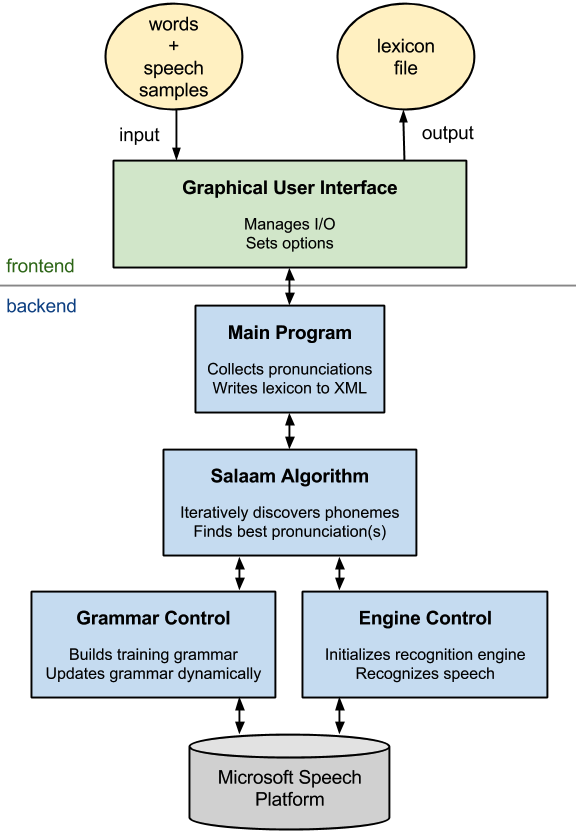
\includegraphics[width=\columnwidth]{../img/SystemOverview-compact.png}
\caption{Overview of the core components of the lex4all lexicon-building application.\label{fig:system}}
\end{center}
\end{figure}

A simple graphical user interface (GUI) allows the user to easily specify one written form (text string) and and one or more audio samples (\texttt{.wav} files) for each term in the target vocabulary.
%, as well as to set other options (detailed in \S\ref{sec:options}). 
Given this input, the program uses the Salaam phoneme-mapping algorithm \cite{Qiao10,Chan12} to find the best pronunciation(s) for each word in the LRL vocabulary. This algorithm requires a pre-trained recognition engine for a HRL (we use American English) as well as a series of dynamically-created recognition grammars. The engine and grammars are constructed and managed using the Microsoft Speech Platform speech recognition libraries \cite{mspsdk}, which are therefore crucial prerequisites for the lex4all application. It should be noted here that in order to make the system more time-efficient, our implementation of Salaam deviates somewhat from the algorithm described by \newcite{Qiao10}; this is discussed further in \S\ref{sec:backend}. 

Once pronunciations for all terms in the vocabulary have been generated, the application outputs a pronunciation lexicon for the given terms as an XML file conforming to the standard pronunciation lexicon specification \cite{pls}, an example of which is given in Listing~\ref{lst:lexicon}. This lexicon can then be directly included in a speech recognition application built using the Microsoft Speech Platform API or a similar toolkit.




%Listing~\ref{lst:lexicon} shows a sample lexicon XML file conforming to the Pronunciation Lexicon Specification \cite{pls}. A lexicon is composed of one \texttt{lexeme} element for each term-sound pairing. In a lexicon intended for speech recognition, each \texttt{lexeme} consists of one \texttt{grapheme} element, representing the term's orthographic form, and one or more \texttt{phoneme} elements, each containing a sequence of phonemes that constitutes an acceptable pronunciation of the term. 

\lstset{
	%language=xml,
	basicstyle={\footnotesize\ttfamily},
	%frame=tb,
	numbers=none,
	linewidth=\columnwidth,
	breaklines=true,
	captionpos=b,
	}
\begin{figure}
\begin{lstlisting}[caption=Example lexicon file mapping the Yoruba word \textit{beeni} (``yes'') to two possible sequences of American English phonemes., label=lst:lexicon]
<?xml version="1.0" encoding="utf-8"?>
	  
<lexicon version="1.0" xmlns="http://www.w3.org/2005/01/pronunciation-lexicon" 
	xml:lang="en-US" 
	alphabet="x-microsoft-ups">
		 
  <lexeme>
    <grapheme>beeni</grapheme>
    <phoneme>B E NG I</phoneme>
    <phoneme>TODO:ANOTHER PRON</phoneme>
  </lexeme>
  
</lexicon>
\end{lstlisting}
%\label{lst:lexicon}
\end{figure}



\section{Pronunciation mapping}
\label{sec:backend}

\subsection{Recognition engine}
\label{sec:engine}
As described above, lex4all uses a recognition engine trained for a HRL to map audio in the target LRL to pronunciations (phoneme sequences) in the source HRL. 
In the current implementation, we use the English (US) speech recognition engine developed by Microsoft for server-side recognition of telephone-quality audio, accessed via the Microsoft Speech Platform SDK 11 \cite{mspsdk}. 
In keeping with the overall objective of the Salaam approach, the engine is used as-is, with no modifications to its underlying models. 
We choose the Microsoft Speech Platform for its robustness and ease of use, as well as to maintain comparability with the work of \newcite{Qiao10} and \newcite{Chan12}, who also used Microsoft's server-side American English recognizer. 
We use an engine designed to recognize low-quality audio since we aim to enable the creation of useful applications for LRLs, including those spoken in developing-world communities, and such applications will most likely need to cope with low-quality audio, e.g. for telephone-based deployment (see e.g. \newcite{case4st4d}).



\subsection{Implementation of the Salaam method}
\label{sec:implementation}

Pronunciations for each term in the target vocabulary are generated using the iterative Salaam algorithm of \newcite[\S4.1]{Qiao10}, described in \S\ref{sec:background} above. In our implementation, 
%we follow \newcite[p. 2]{Chan12} in taking all sequences returned in a given pass as input for the following pass, and 
%we slightly modify the algorithm's stopping condition to terminate 
we stop iterations
if the top-scoring phoneme sequence for a given word has not changed for three consecutive iterations, or -- following \newcite[p. 4]{Qiao10} --  if the best result from the $i^{th}$ pass has a lower score than the best result of the ${i - 1}^{th}$ pass (with the ${i - 1}^{th}$ results returned as the best pronunciations). In both cases, at least three passes are required. 

To determine the best pronunciation sequences for a given term from each pass, the results for all training samples of that term are naively combined into a set, and sorted by the confidence score assigned to each pronunciation (phoneme sequence). If a given pronunciation matches more than one sample, the overall score for that sequence in that pass is simply the sum of confidence scores for all samples it was associated with. In future work, it may be worth exploring more intelligent heuristics for ranking the set of sequences (see \S\ref{sec:future}).

After the iterative training has completed, the $n$-best pronunciation sequences (with $n$ specified by the user -- see \S\ref{sec:options}) for each term are written to the lexicon, each comprising a \texttt{phoneme} element corresponding to the single \texttt{grapheme} element containing the word's orthographic form (e.g. Listing~\ref{lst:lexicon}).

\subsection{Running time}
\label{sec:runningtime}

A major challenge we faced in engineering a user-friendly application based on the Salaam pronunciation-mapping algorithm \cite{Qiao10} was the long running time of the algorithm. As described in \S\ref{sec:background}, the algorithm described by \newcite{Qiao10} depends on a ``super-wildcard'' grammar that allows the recognizer to match the training audio sample to a ``phrase'' of 0-10 ``sub-words'', and each sub-word to any possible sequence of 1, 2, or 3 source-language phonemes. Given the 40 phonemes of American English, this results in 64,000 possibilities for each sub-word, which results in a huge training grammar and thus a long processing time. For a 25-word vocabulary with 5 training audio samples per word, we found the lexicon-building process to take approximately 1-2 hours. This is well beyond the amount of time that a developer will wish to spend creating just one component (the lexicon) of their speech-driven application, especially for a meager 25-word lexicon. 

Therefore, we limit the length of each sub-word in the grammar to only one phoneme, instead of up to 3, giving e.g. 40 possibilities for each sub-word instead of the previous 64,000. Despite the shorter sub-word sequences, this implementation of the algorithm can nonetheless still discover pronunciation sequences of an arbitrary length, since, in each iteration, the phonemes discovered so far are prepended to the super-wildcard grammar, just as before \cite[p.~4]{Qiao10}. However, using this new implementation, constructing the same 25-word vocabulary with the same 5 samples per word takes approximately 2-5 \textit{minutes}. The new implementation is thus an order of magnitude faster than the old implementation.

To ensure that the new implementation's vastly improved running time does not come at the cost of reduced recognition accuracy using the resulting lexicon, we evaluate and compare word recognition accuracy rates using lexicons built with the old and new implementations. The data we use for this evaluation is a subset of the Yoruba data collected by \newcite[\S5.1]{Qiao10}, comprising 25 Yoruba words uttered by 2 speakers (1 male, 1 female), with 5 samples of each word per speaker. 
To determine same-speaker accuracy for each of the two speakers, we perform a leave-one-out evaluation on the five samples recorded per word per speaker (this amounts to a five-fold evaluation, reserving one sample per word per speaker for testing, and training on the other four). Cross-speaker accuracy is evaluated by training the system on all five samples of each word recorded by one speaker, and testing on all five samples from the other speaker.
Using R\footnote{\url{http://www.r-project.org/}} we perform a paired two-tailed $t$-test on the results to assess the significance of the difference in accuracy in each condition.

The results of our evaluation, given in Table~\ref{tab:accuracy}, indicate no statistically significant difference between the accuracy obtained using the old and new implementations (all $p$-values are well above any reasonable significance threshold). Therefore, by making this small modification to the wildcard grammar used for pronunciation discovery, we achieve an implementation of the Salaam algorithm that is much faster than the original, yet yields just as high recognition accuracy. The lex4all application therefore uses the new implementation by default, although for research purposes we leave users the option of using the original (slower) implementation (see \S\ref{sec:options}).

\begin{table}
\begin{center}
\begin{tabularx}{\columnwidth}{X r r r}
\hline
 & Old & New & $p$-value\\
\hline
\addlinespace
\textit{Same-speaker results} & & & \\
\addlinespace
Female  (avg.) & 72.8 & \textbf{73.6} & 0.75 \\
Male  (avg.) & \textbf{90.4} & \textbf{90.4} & 1.00\\
Overall average & 81.6 & \textbf{82} & 0.81 \\
%\hline
%\end{tabularx}
%\end{center}
\addlinespace
%\begin{center}
%\begin{tabularx}{\columnwidth}{X r r r}
\hline
\addlinespace
 \textit{Cross-speaker results} &  &  & \\
 \addlinespace
% \hline
 Train male, test female & \textbf{70.4} & 66.4 &\\
Train female, test male & 76.8 & \textbf{77.6} &\\
 Average & \textbf{73.6} & 72 & 0.63\\
 \addlinespace
\hline
\end{tabularx}
\end{center}
\caption{Difference in word recognition accuracy in Yoruba 
%(25~words, 2~speakers, 5~samples per word per speaker) 
using old (slower) and new (faster) implementations, with $p$-values from 
%paired two-tailed 
$t$-tests. \label{tab:accuracy}}
\end{table}

%\begin{table*}[t]
%\begin{center}
%
%\begin{tabular}{lrccrr}
%%{
%%\toprule
% &  & \multicolumn{2}{c}{Word Recognition Accuracy (\%)} & Difference & $p$-value \\
%\cmidrule(rl){3-4}
%& & Old wildcard & New wildcard & &  \\
%\midrule
%\addlinespace
%Same-speaker & Female (avg.) & 72.8 & \textbf{73.6} &+0.8 & 0.75 \\
%(leave-one-out)		& Male (avg.) & \textbf{90.4} & \textbf{90.4} & 0.0 & 1.00 \\
%			& Overall average & 81.6 & \textbf{82} &  +0.4 & 0.81 \\
%\addlinespace
%\addlinespace
%
%%\midrule
%\addlinespace
%Cross-speaker	&Male $\rightarrow$ Female & \textbf{70.4} & 66.4 & -4.0 & \\
%(train $\rightarrow$ test)		& Female $\rightarrow$ male & 76.8 & \textbf{77.6}& +0.8	&  \\
%			&Average & \textbf{73.6} & 72 	&-1.6	& 0.63 \\
%\addlinespace
%%\addlinespace
%\midrule
%%}
%\end{tabular}
%\end{center}
%\caption{Word recognition accuracy using American English recognizer on Yoruba audio (25~words, 2~speakers, 5~samples per word per speaker), with results of paired two-tailed $t$-test for significance.\label{tab:accuracy}}
%\end{table*}



\subsection{Discriminative training}
\label{sec:discrimtrain}
We implement the iterative discriminative training algorithm of \newcite{Chan12} and offer it as an optional step in the lexicon-building process. In each iteration, this algorithm takes as input the set of mapped pronunciations generated using the Salaam algorithm \cite{Qiao10}, simulates recognition of the training audio samples using these pronunciations, and outputs a ranked list of the pronunciations in the lexicon that best match each sample according to the recognizer. Pronunciations that cause ``confusion'' between words in the vocabulary, i.e. pronunciations that the recognizer matches to samples of the wrong word type, are thus identified and removed from the lexicon, and the process is repeated in the next iteration. \newcite[p.~5]{Chan12} obtain a significant increases in accuracy with up to 8 iterations of the algorithm. lex4all therefore applies this discriminative training (TODO: DEFAULT NUMBER OF PASSES) by default, though users may change the number of passes or disable discriminative training entirely, as mentioned in \S\ref{sec:options}.





\section{User interface}
\label{sec:frontend}

As mentioned above, we aim to make the creation and evaluation of lexicons simple, fast, and above all accessible to users with no expertise in speech or language technologies. Therefore, the application makes use of a simple graphical user interface that allows users to quickly and easily specify input and output file paths, and to control the parameters of the lexicon-building algorithms. 

Figure~\ref{fig:mainform} shows the main interface of the lex4all lexicon builder. This window displays the terms the user has specified and the number of audio samples that the user has selected for each word. Another form, accessed via the "Add word" or "Edit" buttons, allows users to add to or edit the vocabulary by simply typing in the desired orthographic form of the word and selecting the audio sample(s) to be used for pronunciation discovery (see \S\ref{sec:recording} for more details on audio input).


Once the target vocabulary and training audio have been specified, and the additional options have been set if desired, the user clicks the ``Build Lexicon'' button and specifies the desired name and target directory of the lexicon file to be saved. In case of errors (e.g. there are terms in the vocabulary for which no audio files have been specified), a message pops up instructing the user on how to correct the error. Once any errors have been resolved, pronunciation discovery begins, and a progress bar appears above the ``Build Lexicon'' button to keep the user informed of the program's status. When all pronunciations have been generated, a success message displaying the elapsed training time is displayed, and the user may either proceed to the evaluation module to assess the newly created lexicon (see \S\ref{sec:evaluation}), or may return to the main interface to build another lexicon. 

\begin{figure}[tb]
\begin{center}
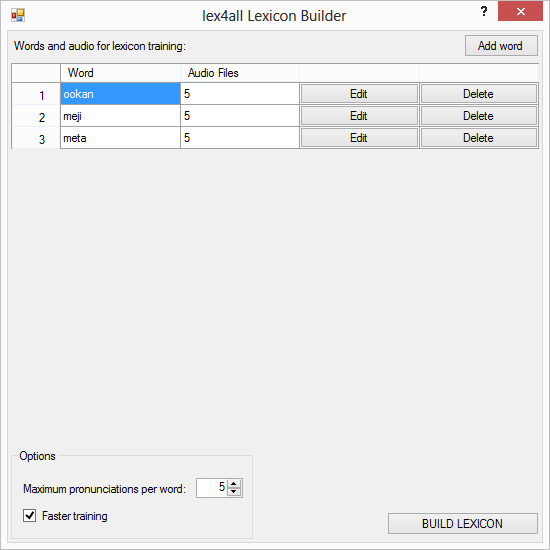
\includegraphics[width=\columnwidth]{../screenshots/LexiconBuilder-Main-Filled.PNG}
\caption{TODO: UPDATE SCREENSHOT Screenshot of the lexicon builder.\label{fig:mainform}}
\end{center}
\end{figure}

\subsection{Audio input and recording}
\label{sec:recording}

%Things to mention (Max, please add to this):
%\begin{itemize}
%\item{NAudio}
%\end{itemize}

%The idea we had in mind was that in addition to uploading existing .wav files it would be interesting to let users record their own audio or ask friends and colleagues to support them. Especially in an international research context such as the one we were developing our tool in that was valuable. 
The GUI allows users to easily browse their file system for pre-recorded audio samples (\texttt{.wav} files) to be used for lexicon training. However, as lex4all has been designed as a language-independent tool, it should enable the development of applications even in zero-resource languages for which no recorded audio is yet available; to this end, the application includes a built-in audio recorder, to simplify the process of collecting audio samples from native speakers.

As the backend for the recording feature we use the open-source library NAudio.\footnote{\url{http://naudio.codeplex.com/}}
% The package offers classes and methods for a variety of audio-related tasks. Essential for us was the access to I/O and volume control, in particular the classes \textit{waveIn}, \textit{waveFileWriter} and \textit{mixerLine}. 
The recorder takes the user's default audio input device as its data source and records one channel with a sampling rate of 8 kHz. 
We use this low sampling rate because the recognition engine we employ is for low-quality audio input (see \S\ref{sec:engine}).
%This fixed setup is due to the fact that we simply prefer low-quality audio because the MS speech recognition aims better results with it.  

A simple GUI form allows users to record audio samples for a given word that has been or is being added to the lexicon vocabulary. Recorded files can be used immediately for lexicon training and/or saved for future use, and can be combined with pre-recorded audio files for training. 

%Although lex4all's audio recording functionality is simple, ...

%Basically two events are handling the input flow. The first one is triggered whenever the record button is not pressed, i.e. whenever the input is not redirected from source to file. Instead it is forwarded to a sample aggregator which stores the maximum volume level of a fixed amount of samples and transmits this value after the amount of samples is reached. The volume level is then displayed on an integrated bar. The reason for the usage of the aggregator is that it would simply overflow the GUI, namely 8000 samples per second. Now we only show 80 samples each second.

%When sound is recorded the data flows straight from the source to a temporary file. Temporary because it is up to the user if we wants to store the file permanently or override it with a subsequent recording. If the first option was chosen the file is also added to the corresponding word as training audio.

\subsection{Additional options}
\label{sec:options}

The lower left corner of the screenshot in Figure~\ref{fig:mainform} shows the parameters and additional options which users can easily modify, if they so choose. First of all, users
%\begin{itemize}
%\item Users 
can specify the maximum number of pronunciations (\texttt{phoneme} elements) that each word in the lexicon may contain. According to \newcite[\S5.2.3]{Qiao10} and \newcite[\S4.2.1]{Chan12}, a higher number of pronunciations per word in the lexicon may improve the resulting recognition accuracy.

%\item Users 
Secondly, we give users the choice of training the lexicon using our modified, much faster implementation of the Salaam algorithm instead of an implementation more closely following \newcite{Qiao10}, as explained in \S\ref{sec:backend}.

%\item Users 
Finally, as mentioned in \S\ref{sec:discrimtrain}, users may choose whether or not discriminative training 
%algorithm of \newcite{Chan12} 
is applied, and if so, how many passes are run.
%\end{itemize}

We make these options easily modifiable via the graphical interface for users who wish to fine-tune the lexicon-building process, possibly to experiment with different settings to achieve the highest possible recognition accuracy. In conjunction with the application's evaluation module (see \S\ref{sec:evaluation}), this expedites further research into language-independent small-vocabulary recognition. However, users who do not wish to change the default settings (shown in Figure~\ref{fig:mainform}) may simply ignore these controls.



\section{Evaluation module for research}
\label{sec:evaluation}

In addition to its primary utility as a lexicon-building tool, lex4all is also a valuable research aide thanks to an evaluation module that allows users to quickly and easily evaluate the lexicons they have created. The evaluation tool allows users to browse their file system for an XML lexicon file that they wish to evaluate; this may be a lexicon created using lex4all, or any other lexicon conforming to same format \cite{pls}. The application reads this lexicon and automatically populates a list of its words (\texttt{grapheme} elements), displaying them in a window similar to that of Figure~\ref{fig:mainform}; users may remove words from the evaluation set, but may not add any words that are not included in the lexicon file. As in the main interface, users then select one or more audio samples (\texttt{.wav} files) for each word, which will be used for testing. At the click of a button, the system attempts to recognize each of the given audio samples using the given lexicon, and then reports the number of samples correctly and incorrectly recognized, and the number (if any) that could not be recognized. Users may optionally save this report, along with a confusion matrix of word types, as a comma-separated values (\texttt{.csv}) file, which can be easily imported into standard spreadsheet or statistical analysis software for analysis of the results. 

This evaluation tool thus allows users to quickly and easily assess different configurations of the lexicon-building tool, by simply changing the settings using the GUI (see \S\ref{sec:options}) and evaluating the resulting lexicons. Furthermore, as the application's source code is freely available and modifiable, researchers may even replace entire modules of the system (e.g. use a recognition engine for a different source language, or a different pronunciation-discovery algorithm), and use this evaluation module to quickly assess the results. This tool therefore greatly facilitates further research into language-independent small-vocabulary speech recognition. 

\section{Conclusion and future work}
\label{sec:future}

We have presented lex4all, an open-source Windows desktop application that enables the rapid automatic creation of pronunciation lexicons in any (low-resource) language, using an out-of-the-box commercial recognizer \cite{mspsdk} for a high-resource language (English) and the Salaam method for cross-language pronunciation mapping \cite{Qiao10,Chan12}. The application thus makes small-vocabulary speech recognition interfaces feasible in any language, since the algorithm requires only minutes of training audio; combined with the built-in audio recorder, lexicons can be constructed even for zero-resource languages. We hope that this tool will help developers create speech-driven applications in LRLs, as well as facilitate research in language-independent small-vocabulary recognition.

Future directions for the development of lex4all include the addition of more back-end options to give users even greater control over the lexicon-building process. One logical next step would be to expand the selection of source-language recognizers; at the moment, lex4all only offers American English as the source languge, but any of the 20+ other high-resource languages supported by the Microsoft Speech Platform \cite{mspsdk} could theoretically be used, and it would be interesting to investigate different pairings of source and target languages. Another future goal is to improve and extend the functionality of the audio-recording feature (see \S\ref{sec:recording}), 
%by giving users greater control over e.g. the sampling rate for recordings, and/or by making the tool more user-friendly with e.g. instant playback of recorded audio. 
to make the recording tool more flexible and user-friendly.
Finally, as an extension of the lex4all project, it would be beneficial to offer users the option to share the lexicons they have built and the speech samples they have recorded by uploading this data to a central online repository. Over time, this could become a valuable collection of data for LRLs, enabling developers and researchers to share and re-use data among languages or language families.

% future work on the recording function
%It would be advantageous to display the volume while recording which is at the moment not possible because data is redirected either way. Unfortunately we had issues when doing both simultaneously which resulted in disturbances in the recorded audio.
%A major advantage would it be to play back what has been recorded, so the user does not have to save the file first in order to check its quality and content.

%\section*{Acknowledgments}
%
%The acknowledgments should go immediately before the references.  Do
%not number the acknowledgments section. Do not include this section
%when submitting your paper for review.

% include your own bib file like this:
%\bibliographystyle{acl}
%\bibliography{acl2014}
\bibliographystyle{acl}
\bibliography{lex4all.bib}


\end{document}
